\chapter{Materials and Methods}\label{chap:materials-methods}
This chapter introduces the materials and datasets provided in the source paper \citep{Ferber2024}. We then describe how the data were preprocessed and explored, explain how the models were implemented, trained, and evaluated, and finally present the methods used to analyse model explainability.

\section{Data and Materials}\label{sec:method-data-materials}
As part of \citet{Ferber2024}, the authors have published a dataset of 1798 \glspl{subject} running or walking on a treadmill captured using multi-camera 3D \gls{mocapsys}. The dataset is composed of raw 3D~marker data of each \gls{session}, descriptive biomechanical variables derived from the marker data for each session and demographic and anthropometric metadata of the subjects. Additionally, the matlab code for the preprocessing of the data, the calculation of the kinematic variables and tutorial notebooks that help lustrate how to use their library and read the data from the folder structure are also provided. Although both walking and running data is provided, we have used exclusively running data. From this point onwards, walking data is ignored for brevity.

\subsection{Measurement protocol}\label{subsec:measurement-protocol}
The complete measurement protocol is described in \citet{Ferber2024}. In this subsection, we provide a summary of the aspects that are most relevant for the methods and analyses presented in this thesis.

The raw marker data was collected using high-speed optoelectronic infrared-based motion capture cameras (MX3/Bonita, Vicon, Oxford, UK) were used to record the position of 9~mm spherical retro-reflective markers attached to anatomical landmarks of the subjects at either 120~Hz or 200~Hz. Depending on the lab, eight or three cameras were used. Below we list and describe the three sets of markers that were used.
\begin{itemize}
    \item \textbf{Core}: Markers attached to the following anatomical landmarks: medial and lateral malleoli, medial and lateral femoral condyles, and greater trochanters.
    \item \textbf{Additional}: Markers attached to the following anatomical landmarks: bilateral 1st and 5th metatarsal heads, distal aspect of the shoe, tibial tuberosity, anterior superior iliac spines, and iliac crests;
    \item \textbf{Clusters}: 3 or 4 markers placed on rigid shells attached to the following anatomical landmarks: sacrum, bilateral thigh and shank, and posterior aspect of both shoes.
\end{itemize}

During the recording of the sessions of all 1798 subjects the 'core' and 'cluster' set of markers were used. The additional set was only used during the recording of the sessions of 1082 subjects. Figure \ref{fig:marker_position} shows the lower body of a subject and the three sets of markers.

\begin{figure}[ht]
    \begin{centering}
    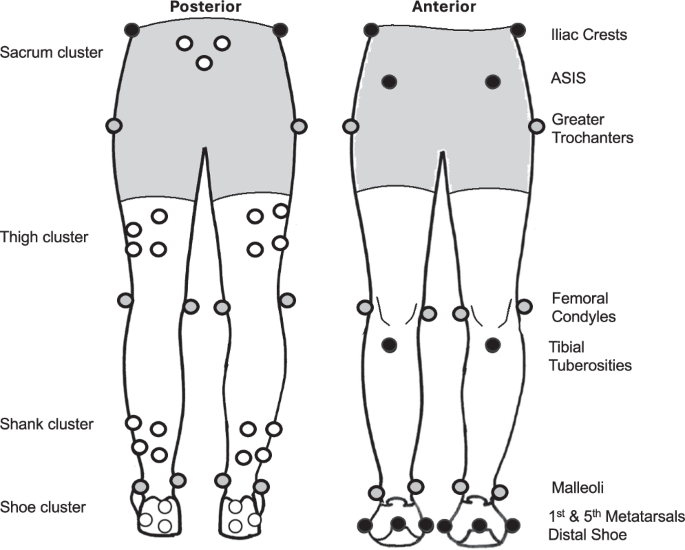
\includegraphics[width=0.5\columnwidth]{images/billateral_marker_position.png}
    \par\end{centering}
    \caption{Position of markers on the subjects. Grey markers correspond to core set of markers set, black to additional set and white to the clusters set.}
    \label{fig:marker_position}
\end{figure}

% TODO: Explain the recording procedure: Warm up, duration, discard, etc...

\subsection{Dataset Description}\label{subsec:method-dataset-description}
As described above, the dataset contains two complementary components: (i) session-level metadata stored as tabular files, and (ii) motion-capture marker data together with derived kinematic variables per session. Below we describe each component and list the variables that are available for analysis.

\paragraph{Metadata File (tabular)} The metadata file is provided as a CSV file: \texttt{run\_data\_meta.csv}. Each row corresponds to a single treadmill session recorded for a subject. It contains anthropometric and demographic variables.
\begin{itemize}
    \item \texttt{sub\_id}: Unique subject identifier.
    \item \texttt{datestring}: Session recording date.
    \item \texttt{filename}: Session filename used to locate the marker json file for the session.
    \item \texttt{speed\_r}: Treadmill belt speed (m/s).
    \item \texttt{age}: Subject's age (years).
    \item \texttt{Height}: Body height (cm).
    \item \texttt{Weight}: Body weight (kg).
    \item \texttt{Gender}: Subject gender.
    \item \texttt{DominantLeg}: Dominant leg (Left/Right/Ambidextrous).
    \item \texttt{InjDefn}: Injury severity reported by the subject choosing between 4 options: (1) No Injury, (2) Continuing to train in pain, (3) Training volume/intensity affected, (4) Minimum of two workouts missed in a row.
    \item \texttt{InjJoint}, \texttt{InjSide}, \texttt{SpecInjury}, \texttt{InjDuration}: Primary injured joint, side (Left/Right), Specific injury diagnosis from medical professional, and for how long has the subject had the injury.
    \item \texttt{InjJoint2}, \texttt{InjSide2}, \texttt{SpecInjury2}: Secondary injury information (if applicable).
    \item \texttt{Activities}: Subject reported athletic activities performed on a regular basis.
    \item \texttt{Level}: Self-reported level of athletic activity (recreational/competitive).
    \item \texttt{YrsRunning}: Number of years subject has been running on a regular basis.
    \item \texttt{RaceDistance}: Preferred race distance.
    \item \texttt{RaceTimeHrs}, \texttt{RaceTimeMins}, \texttt{RaceTimeSecs}: Preferred race distance best time.
    \item \texttt{YrPR}: Year of preferred race distance personal best time.
    \item \texttt{NumRaces}: Number of races completed per year.
\end{itemize}

\paragraph{Marker and descriptive biomechanical data (Hierarchical)} For each session, 3D positions of reflective markers and descriptive variables derived from those markers are provided as json files. One file per session.
\begin{itemize}
    \item \textbf{Recording frequency} Frequency of the recording in Hertz (Hz). Either 120 Hz or 200 Hz depending on the lab.
    \item \textbf{Joint Marker Neutral}: 3D coordinates of the individual markers of the core and additional marker sets while the subject is standing in neutral position.
    \item \textbf{Cluster Marker Neutral}: 3D coordinates of the individual markers in the cluster marker set while the subject is standing in neutral position.
    \item \textbf{Dynamic Marker data}: 3D coordinates at each of the frames of the recording for the individual markers in the cluster marker set.
    \item \textbf{Descriptive biomechanical variables}: Set of 77 variables derived from the 3D coordinates Marker data. Calculated for Left and Right side of the body.
\end{itemize}

It must be noted that \texttt{Joints} and \texttt{Neutral} coordinates do not represent the true anatomical centres, only the centres of the markers on the skin of the subject.
Only 33 of the 77 descriptive biomechanical variables are populated per side, the rest all contain 0 for all values of all sessions, this totals 66 populated descriptive variables in total. Table \ref{tab:met-desc-variable-init} describes the variable set per side.

\begin{table}[ht]
    \centering
    \caption[Populated Descriptive Variables Summary]{Summary of the Descriptive Biomechanical Variables that are populated\label{tab:met-desc-variable-init}}
    \begin{tabular}{lp{0.6\textwidth}}
    \hline
    \textbf{Variable} & \textbf{Category} \\
    \hline
    Step width (m) & Temporal-spatial \\
    Stride rate (steps/min) & Temporal-spatial \\
    Stride length (m) & Temporal-spatial \\
    Swing time & Temporal-spatial \\
    Stance time & Temporal-spatial \\
    Peak drop angle & Pelvis kinematics \\
    Drop excursion & Pelvis kinematics \\
    Dorsiflexion peak angle & Ankle kinematics \\
    Ankle Eversion peak angle & Ankle kinematics \\
    Ankle Rotation peak angle & Ankle kinematics \\
    Ankle Eversion excursion & Ankle kinematics \\
    Ankle Rotation excursion & Ankle kinematics \\
    Ankle Eversion \% of stance & Ankle kinematics \\
    Knee Flexion peak angle & Knee kinematics \\
    Knee Adduction/abduction peak angle & Knee kinematics \\
    Knee Rotation peak angle & Knee kinematics \\
    Knee Adduction/abduction excursion & Knee kinematics \\
    Knee Rotation excursion & Knee kinematics \\
    Hip Extension peak angle & Hip kinematics \\
    Hip Adduction peak angle & Hip kinematics \\
    Hip Rotation peak angle & Hip kinematics \\
    Hip Adduction excursion & Hip kinematics \\
    Hip Rotation excursion & Hip kinematics \\
    Foot progression angle & Foot kinematics \\
    Heel-strike angle & Foot kinematics \\
    Medial heel whip excursion from toe-off & Foot kinematics \\
    Ankle eversion peak velocity & Joint velocities \\
    Ankle rotation peak velocity & Joint velocities \\
    Knee adduction peak velocity & Joint velocities \\
    Knee abduction peak velocity & Joint velocities \\
    Hip abduction peak velocity & Joint velocities \\
    Knee rotation peak velocity & Joint velocities \\
    Hip rotation peak velocity & Joint velocities \\
    Pelvic drop peak velocity & Joint velocities \\
    Pronation onset \% of gait cycle & Foot timing \\
    Pronation offset \% of gait cycle & Foot timing \\
    Vertical oscillation (mm) & Vertical oscillation \\
    \hline
    \end{tabular}
\end{table}

All descriptive variables follow the interpretations described in \citet{Bartlett2014}. Unless specified explicitly in the table, the units are degrees for angles and excursions, and degrees/s for joint velocities. Excursions are also commonly known as range of motion (ROM) in the literature. 
% TODO: Explain important biomechanical concepts like dorsiflexion, eversion, etc...

\subsection{Code Description}\label{subsec:method-code-description}
Python was the main language used in this project, although several scripts were implemented in \GLS{matlab} for the data acquisition and extraction stages. Matlab was also used to preprocess the dataset, following the procedure described in the source paper. All code created for this project and used to generate the reported results has been made publicly available for reproducibility \cite{Zapater_Reig_Running_Injury_Clinic_2025}.

The MATLAB reference implementation published with the dataset in \citet{Ferber2024} was employed as part of this work. The corresponding MATLAB scripts have been included in the repository under the \texttt{supplemental\_material} folder for consultation.

The following assets are the most relevant components of the repository:

\paragraph{Notebooks}
\Gls{jupyter} notebooks used during development. These capture the iterative process across the different phases of the project and the reporting of results.

\paragraph{\texttt{core} Package}
Python package containing the core functionality used in the notebooks. It includes classes, functions, and constants to orchestrate data extraction, preprocessing, feature engineering, model training, and evaluation.

\paragraph{\texttt{gait\_kinematics.m}}
Script provided with the source paper. It calculates joint angles and angular velocities from the \texttt{Dynamic Marker Data}, \texttt{Joint Marker Neutral}, and \texttt{Cluster Marker Neutral} files. Anatomical segment coordinate systems are constructed from the neutral marker data, segment motion is tracked using the dynamic marker data, and XYZ Cardan joint angles and angular velocities are computed. The script returns:
\begin{itemize}
    \item \texttt{Angles}: per-frame joint/segment angles for the left/right ankle, knee, hip, as well as foot and pelvis segments (degrees).
    \item \texttt{Velocities}: per-frame angular velocities for the same structures (deg/s).
    \item \texttt{jc}: estimated joint centre positions (pelvis, hips, knees, ankles).
\end{itemize}

\paragraph{\texttt{gait\_steps.m}}
Script also provided with the source paper. It calculates descriptive biomechanical variables from the \texttt{Dynamic Marker Data}, \texttt{Cluster Marker Neutral}, \texttt{Angles}, and \texttt{Velocities}. The script returns:
\begin{itemize}
    \item \texttt{event}: gait cycle events by side (touchdown, mid-stance, toe-off, heel whip).
    \item \texttt{Descriptive biomechanical variables}: as defined in Table~\ref{tab:met-desc-variable-init}.
\end{itemize}

\paragraph{\texttt{processing\_source\_data.m}}
Script implemented for this project to process the metadata file and marker-data JSON files. Joint angles, joint angular velocities and cycle events are computed by calling \texttt{gait\_kinematics.m} and \texttt{gait\_steps.m}. The outputs are converted into tabular format for the exploratory data analysis (EDA) stage.


\subsection{Data Extraction}\label{subsec:data-extraction}

The script \texttt{processing\_source\_data.m} was executed to process the raw dataset. Out of 2506 recorded sessions (with some subjects contributing multiple sessions), 2487 were processed successfully, of which 1813 contained valid running data. Sessions without running data or those where MATLAB preprocessing failed were excluded.

The outputs consist of time-series data for markers, joint angles, joint angular velocities, and detected gait cycle events with their corresponding frame indices. These outputs were further processed using the \texttt{pandas} and \texttt{kinetics-toolkit} Python packages to combine the event information with the time-series data.

Figure \ref{fig:data-ext-marker-velo-angle-ts} illustrates an example from a single session, showing the raw marker data for one marker in the left shank cluster together with the corresponding joint angle and angular velocity for the left knee. Figure \ref{fig:data-ext-l-knee-angle-events} shows frames 500--1000 of the left knee angle, annotated with the touchdown and toe-off events. Figure \ref{fig:data-ext-marker-3d} provides a 3D representation of a frame with the full marker set.

In addition to the time-series data, the script also generates the a of 33 descriptive variables. These variables are equivalent to those stored in the JSON files of the source dataset. To validate the execution of \texttt{processing\_source\_data.m}, the generated variables were compared against the source dataset. All variables matched within a relative tolerance of $1 \times 10^{-9}$, except for 35 values of \texttt{speed\_r}, which differed by $9 \times 10^{-2}$. This deviation is negligible when measuring human running speed in m/s and confirms that the execution was successful. The resulting data was considered ready for the exploratory data analysis stage.

\begin{figure}[ht]
    \centering
    \begin{minipage}[t]{0.48\textwidth}
        \centering
        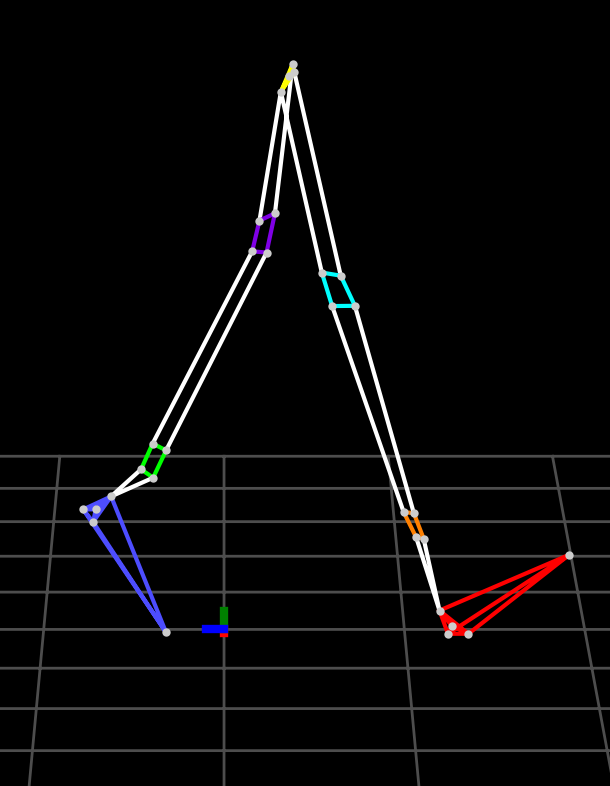
\includegraphics[width=\textwidth]{images/ex_3d_marker.png}
        \caption{3D representation of a frame with all marker data. Connecting lines have been added between markers. The left foot is coloured blue and the right foot red. From top to bottom: pelvis, left/right thigh, left/right shank, and left/right foot.}
        \label{fig:data-ext-marker-3d}
    \end{minipage}
    \hfill
    \begin{minipage}[t]{0.48\textwidth}
        \centering
        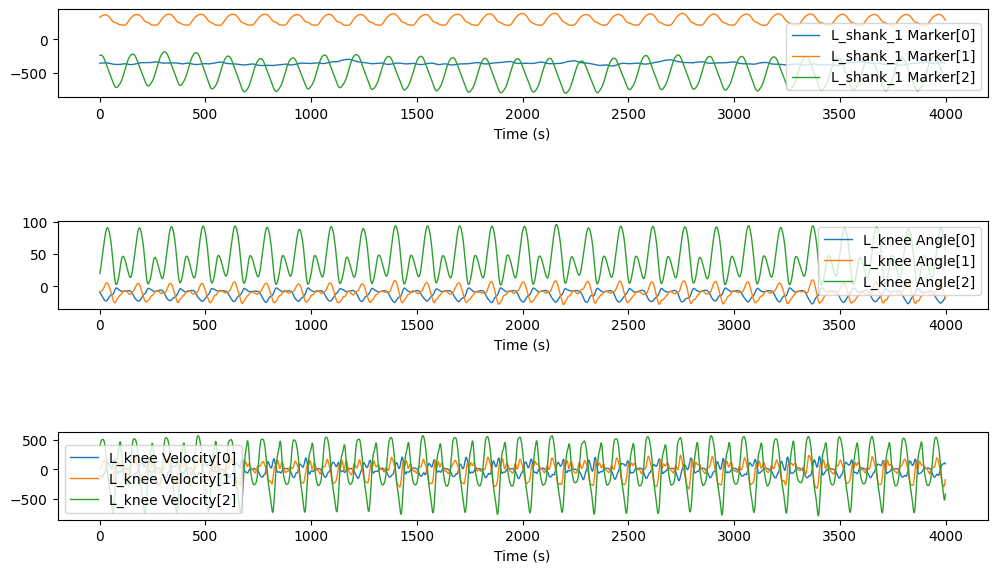
\includegraphics[width=\textwidth]{images/ex_marker_angle_vel_ts.png}
        \caption{Example time series from a single session showing the first left shank marker, left knee angle, and left knee angular velocity across the three axes: [0] X, [1] Y, [2] Z.}
        \label{fig:data-ext-marker-velo-angle-ts}
    \end{minipage}
\end{figure}

\begin{figure}[ht]
    \centering
    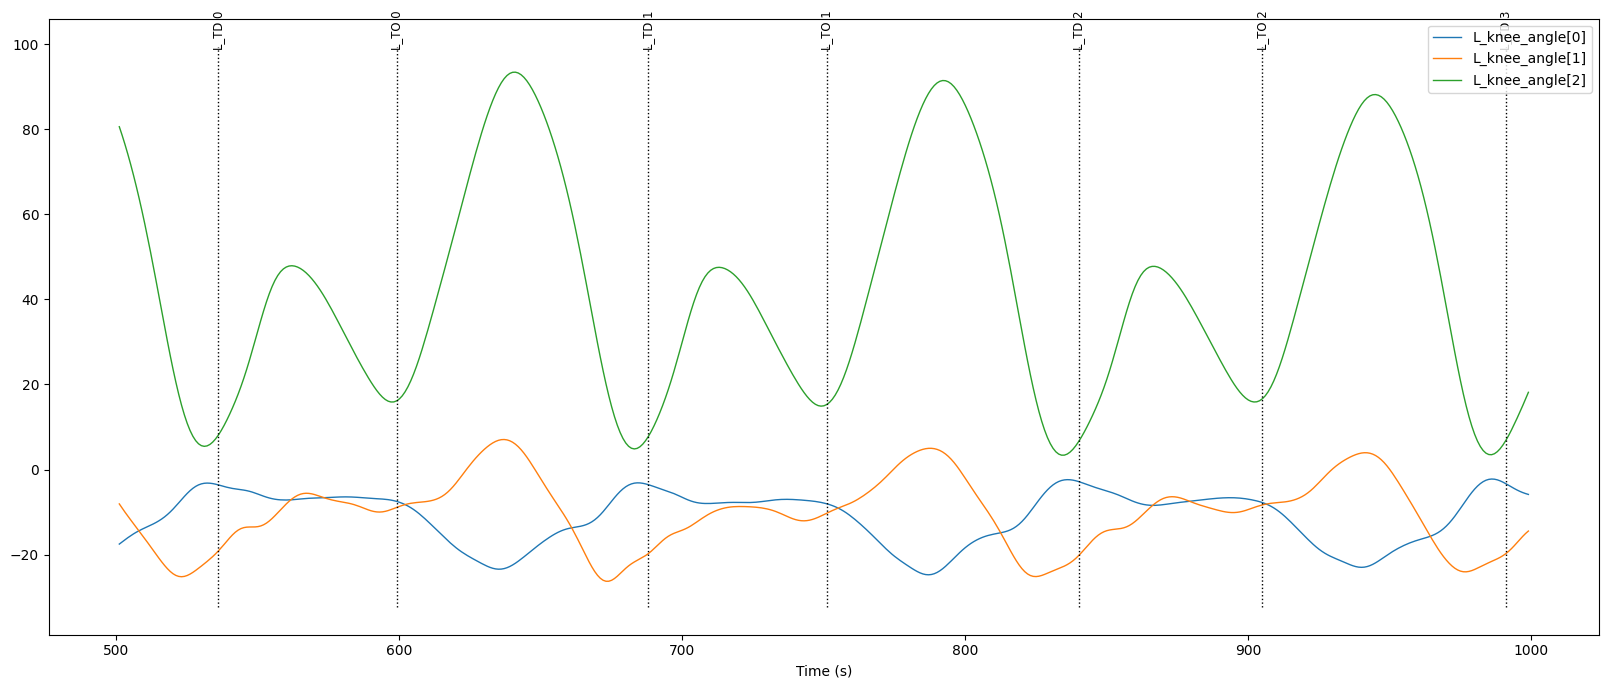
\includegraphics[width=0.5\columnwidth]{images/ex_l_knee_angle_events.png}
    \caption{Frames 500--1000 of the left knee angle (three axes: [0] X, [1] Y, [2] Z), annotated with touchdown (\(L\_TD\)) and toe-off (\(L\_TO\)) events.}
    \label{fig:data-ext-l-knee-angle-events}
\end{figure}


% TODO: End with a summary of the tabular and time-series data that we have extracted?

\section{Exploratory Data Analysis (EDA)}\label{sec:method-eda}
% -- Exploration → Extraction → Preparation, with concrete checks and figures:
% -- Tabular data Exploration (sanity and distributions)
% -- Dataset inventory (sessions per runner, class prevalence per runner, cycles/session).
% -- Missing-ness map (metadata \& signals); strategy preview (drop/impute).
% -- Outliers: per-joint angle/velocity ranges, z-score >3 heat-map by runner (flag sensors/markers).
% -- Dimensionality previews: PCA/t-SNE to see separability.
As discussed on the previous section, we have two main types of data available:

\begin{itemize}
    \item \textbf{Tabular datasets}
    \begin{itemize}
        \item Session metadata, a set of anthropometric and demographic variables.
        \item Descriptive variables, a engineered set of biomechanical variables derived from the joint angles and angular velocities.
    \end{itemize}
    \item \textbf{Time-series datasets}
    \begin{itemize}
        \item Joint angles derived from the marker data.
        \item Joint angular velocities derived from the marker data.
    \end{itemize}
\end{itemize}

Given the difference in structure of both groups of datasets we need to apply different techniques and methods when working with them. Below we will discuss each of them separately.

\subsection{Tabular dataset}\label{subsec:method-tabular-dataset}
The tabular datasets contain a row for each of the 1813 recordings of running sessions. There are 1394 distinct runners within those sessions, with 207 of them having more than 1 session recorded.

\paragraph{Categorical Variable Cleaning and Encoding}
The values of nominal categorical variables with less than 100 categories have been mapped to a code that is easier to work with(no spaces, no special characters and restricted length), and we have consolidated categories that refer to the same code but were written slightly differently (i.e. meniscal tear-lateral and meniscal tear lateral).

For nominal categorical variables with more than 100 categories that are likely a free text input for the subjects like \texttt{Activities}, we Convert to lowercase, remove leading and trailing spaces, replace non-standard separators with comma, replace multiple spaces with single space, replace multiple commas with single comma.

For ordinal categorical values, we have introduced both a code and a numerical representation so that we can choose what to use depending on the task.
Quantitative variables have been left unchanged, standardisation and normalization has been left for a later stage.

All values that do not fall into a defined category or an accepted value for the data-type are considered as missing value and are converted to None. This is saved as "" when saving the dataset to CSV format.

> TODO: Expand each of the points and add visualization if needed.

Key points regarding the distributions of the columns:
\begin{itemize}
    \item The male/female distribution is balanced (exact percentage to be reported), with few empty values.
    \item The \texttt{DominantLeg} variable is skewed towards the right leg, as expected; there are few ambidextrous cases.
    \item The distributions of \texttt{SpecInjury} and \texttt{InjDefn} are noteworthy and should be reported.
    \item The "Level" variable (recreational vs. competitive) is skewed towards recreational runners.
    \item There is little longitudinal data: only 30 sessions (2.1\%) are at least one month apart.
\end{itemize}

\paragraph{Data Quality and Outlier detection}
During inspection of the dataset, several inconsistencies were identified. In some cases, the level of athletic activity (\texttt{Level}), the reported dominant leg (\texttt{DominantLeg}), and the injury descriptors (\texttt{SpecInjury} and \texttt{InjDefn}) changed across sessions for the same subject. These cases were considered plausible and interpreted as part of the natural variability of the dataset. No indication was found in the source paper that such cases should be regarded as data quality issues, and they were therefore left unchanged.

One case was found in which the reported age differed by ten years between two sessions, which exceeds the duration of the study. To investigate, the entire dataset was checked for inconsistencies between reported age and the time difference between sessions. Two problematic cases were identified:
\begin{itemize}
    \item Subject 100234 was recorded as 40 years old in the first session and 43 years old one year later. In this case, the age in the second session was corrected to 41.
    \item Subject 200375 was recorded as a 27-year-old female in one session and as a 50-year-old male in the next. This inconsistency suggests that the sessions belong to different individuals. A new synthetic subject identifier (300375) was therefore created, and the second session was reassigned to this new subject. The total number of sessions remained unchanged, but the number of unique subjects increased by one.
\end{itemize}

Additional inconsistencies were found in the injury variables. In many sessions, \texttt{SpecInjury} was empty while \texttt{SpecInjury2} contained information. These cases were treated as input errors: when \texttt{SpecInjury} was missing and \texttt{SpecInjury2} was populated, the value of \texttt{SpecInjury2} was taken as the primary injury. A subject was assumed to have no primary injury in a session only if both fields were empty.

All columns in the metadata were inspected for implausible values. Table \ref{tab:met-outlier-range} summarises the range thresholds used for outlier detection. Values outside of these ranges were considered unrealistic and replaced with \texttt{None}. For example, ages of 255~years, heights of 999~cm, weights of 1564~kg, injury durations of 30,000~days (82~years), and years running of 999 were identified as outliers and removed. These extreme values were detected visually using box plots and validated against plausible ranges for human adults.


%TODO: Try to get it to show together with the text
\begin{table}[htbp]
    \centering
    \caption[Outlier detection range for tabular data]{Summary of outlier detection ranges for key variables.\label{tab:met-outlier-range}}
    \begin{tabular}{lcc}
        \hline
        \textbf{Variable} & \textbf{Min} & \textbf{Max} \\
        \hline
        Age & 18.0 & 73.0 \\
        Height (cm) & 120.0 & 196.5 \\
        Weight (kg) & 42.5 & 176.0 \\
        Injury duration (days) & 0.0 & 176.0 \\
        Years running & 0.0 & 54.0 \\
        \hline
    \end{tabular}
\end{table}


\paragraph{Merging metadata and biomechanical variables} 
A surrogate key \texttt{id} was introduced to uniquely identify each sample across datasets, where one sample corresponds to a session. The surrogate key was defined as the concatenation of the subject identifier and the session filename in uppercase (e.g., \texttt{100001\_20110531T161051}). This column was then used as the join key to merge the metadata and biomechanical variables.
% TODO: List all variables available? Maybe better on a Apendinx?

\paragraph{Missing values}
Table\ref{tab:met-missing-values} presents the ten variables with the highest proportion of missing values after standardisation, data cleaning, and outlier detection. We decided to keep all discrete variables and \texttt{age}, \texttt{Height}, \texttt{Weight}, \texttt{Gender} and \texttt{DominantLeg}.

For numeric variables, the maximum proportion of missing values was 0.7\%. However, dropping all rows with at least one missing value would have removed more than twice as many samples. To preserve data, missing values in numeric variables were therefore imputed with the median. The median was chosen because normality could not be assumed for all variables and several distributions were skewed. Under such conditions, the median is more robust than the mean.

For categorical variables, missing values were replaced with the label \texttt{unknown} to allow easy identification of imputed categories.

\begin{table}[htbp]
    \centering
    \caption[Top 10 metadata variable with most missing values]{Top 10 Variable with the highest percentage of missing values after cleaning.\label{tab:met-missing-values}}
    \begin{tabular}{lc}
        \hline
        \textbf{Column} & \textbf{Missing (\%)} \\
        \hline
        YrPR & 77.16 \\
        RaceTimeSecs & 75.95 \\
        NumRaces & 72.91 \\
        RaceTimeHrs & 70.04 \\
        RaceTimeMins & 62.05 \\
        YrsRunning & 31.16 \\
        DominantLeg & 19.46 \\
        RaceDistance & 18.64 \\
        Activities & 17.42 \\
        Level & 14.83 \\
        \hline
    \end{tabular}
\end{table}


\paragraph{Definition of Injury status}
Seven columns contain injury data: primary injury data (\texttt{SpecInjury}, \texttt{InjJoint}, \texttt{InjSide}), secondary injury data (\texttt{SpecInjury2}, \texttt{InjJoint2}, \texttt{InjSide2}), and injury severity (\texttt{InjDefn}), and while primary and secondary injury data is consistent within each group, they are not consistent with injury severity. In total, 9\% of the dataset wither was diagnosed with no injury but the runner reported, at least, that they were "continuing to train in pain" or was diagnosed with an injury but reported \texttt{"no injury"} in the severity score.

The source paper does not precise clearly what logic did they use for a subject to be counted as uninjured, but we have decided to use the information coming from \texttt{SpecInjury} and \texttt{SpecInjury2} because it is medically diagnosed by a medical practitioner. So if any of these two variables has a value other than \texttt{"no\_injury"}, we will flag the runner as injured during the session. The distribution of injured vs uninjured sessions is 63.5\% to 36.5\%.


\paragraph{Variable standardisation for training}
To prepare the variables for training, numerical values were standardised using the Z-score $Z = (X - \mu) / \sigma$. This procedure centres the data around a mean of 0 and scales it to a standard deviation of 1. Standardisation reduces bias when working with variables of different magnitudes and is required for models such as Logistic Regression and Support Vector Machine (SVM).

Categorical variables were converted into sparse one-hot encoded arrays, where each category value is represented as a separate column and encoded with a 1 or 0 to indicate its presence. To mitigate perfect collinearity, where one variable can be predicted exactly from another, reducing the reliability of coefficient estimates and hindering interpretability, the column corresponding to the value \texttt{unknown} was dropped for each categorical variable.


\paragraph{Analysis of relationship between predictors and target variable}
t-distributed Stochastic Neighbor Embedding (t-SNE) is a non-linear dimensionality reduction technique that projects high-dimensional data into a low-dimensional space while preserving local neighbourhood relationships \citep{JMLR:v9:vandermaaten08a}. In this project, t-SNE was applied as an exploratory tool to assess whether natural clustering exists in the data. Seven plots were generated with different values of the hyperparameter \texttt{perplexity}, and the plot that best reflected the data structure was chosen. The range of perplexity values proposed in \citet{JMLR:v9:vandermaaten08a} as typical was used.

\begin{figure}[ht]
    \centering
    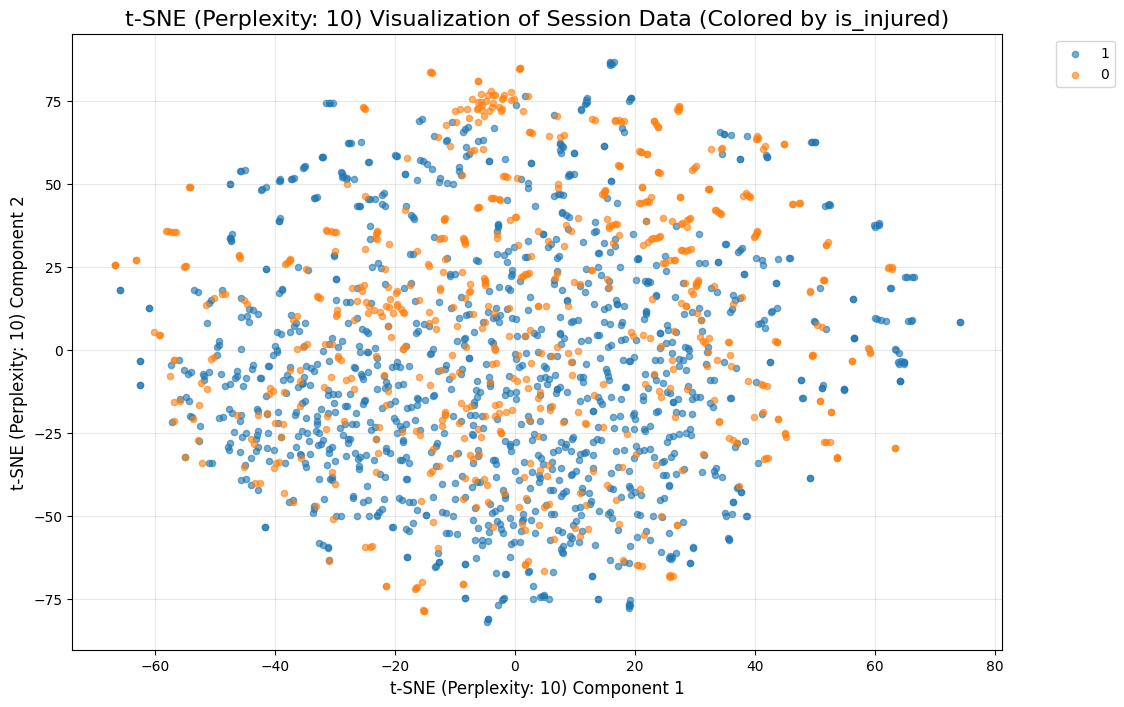
\includegraphics[width=0.5\columnwidth]{images/t-sne-p10-scatter-is_injured.png}
    \caption[2D t-SNE plot with perplexity 10]{2D t-SNE plot with perplexity 10. Injured samples appear in blue and uninjured samples in orange.\label{fig:met-tsne-injured}}
\end{figure}

Figure \ref{fig:met-tsne-injured} shows the 2D t-SNE projection of the cleaned dataset. The embedding suggests that no strong natural groupings exist, as injured and uninjured samples overlap accross most of the plot. A small cluster of uninjured samples is visible in the upper-central region of the plot, but the distance to neighbouring points is limited. This indicates that even the most distinct subgroup is not well separated and that class separation is more complex due to high similarity between classes. It should also be noted that the figure only displays the first two t-SNE components. Additional separation may exist in higher-dimensional representations.

The plot also highlights differences in the relative density of the two classes: injured samples appear more frequently in the lower-left region of the plot, whereas uninjured samples are more common in the upper-center. A separating line could be drawn such that more than 50\% of the uninjured samples fall on one side, suggesting that a simple linear classifier trained on the t-SNE components would perform slightly better than random chance. This indicates that some degree of class separation is present, although it remains weak.

<DRAFT>\dots 
To further analyse the relationship between the predictors and the target variable, we calcualte the mutual informaiton MI, for numerical values we calcualte the pearson correlation and perform a t-test to compare the distributions of the injured and uninjured populations. For categorical data, we perform the ChiSquared test. Table~\ref{tab:met-top-vars-stat-test} shows the top 5 scorers by metric.

MI measures how much knowing a variable reduces uncertainty about the target and it is able to capture non-linear dependencies. Pearson r measures the linear correlation, the sign reflects if the correlation is positive or negative. The t-test compares means of injured and non-injured populations, if $p < 0.05$, the difference between the means is statistically significant. Similarly, the ChiSquared test calculates if the difference in distribution between injured and non-injured populations is statistically significant.

\begin{table}[htbp]
    \centering
    \caption{Top Predictors of Injury Status Across Statistical Tests. \label{tab:met-top-vars-stat-test}}
    \begin{tabular}{lll}
        \hline
        \textbf{Metric} & \textbf{Predictor} & \textbf{Score} \\
        \hline
        \multicolumn{3}{l}{\textit{Top 5 by Mutual Information}} \\
        & weight & 0.069027 \\
        & age & 0.045877 \\
        & height & 0.043159 \\
        & dom\_leg\_foot\_ang\_at\_hs & 0.021200 \\
        & dom\_leg\_diff\_knee\_abd\_peak\_angle & 0.021124 \\
        \hline
        \multicolumn{3}{l}{\textit{Top 5 by absolute correlation with is\_injured}} \\
        & dom\_leg\_stance\_time & Pearson $r$ = 0.228451, $p$ = $6.78 \times 10^{-23}$ \\
        & dom\_leg\_stride\_length & Pearson $r$ = -0.166545, $p$ = $9.58 \times 10^{-13}$ \\
        & dom\_leg\_ankle\_eve\_peak\_vel & Pearson $r$ = 0.149308, $p$ = $1.67 \times 10^{-10}$ \\
        & dom\_leg\_hip\_ext\_peak\_angle & Pearson $r$ = 0.139237, $p$ = $2.62 \times 10^{-9}$ \\
        & dom\_leg\_pelvic\_drop\_peak\_vel & Pearson $r$ = -0.133314, $p$ = $1.21 \times 10^{-8}$ \\
        \hline
        \multicolumn{3}{l}{\textit{Top 5 by t-test p-value}} \\
        & dom\_leg\_stance\_time & $6.78 \times 10^{-23}$ \\
        & dom\_leg\_stride\_length & $9.58 \times 10^{-13}$ \\
        & dom\_leg\_ankle\_eve\_peak\_vel & $1.67 \times 10^{-10}$ \\
        & dom\_leg\_hip\_ext\_peak\_angle & $2.62 \times 10^{-9}$ \\
        & dom\_leg\_pelvic\_drop\_peak\_vel & $1.21 \times 10^{-8}$ \\
        \hline
        \multicolumn{3}{l}{\textit{Top 1 by Chi$^2$ p-value}} \\
        & gender & 0.193481 \\
        \hline
    \end{tabular}
\end{table}

TODO: Explain patterns. Quick summary: In summary t-test and correlation show that, although the value of correlation is small, there is a statistically significant difference between both classes. Gender as expected is not statistically significant. Interesting too see that variables other than the ones with highest correlatin show in MI. This is because MI captures non-linear relationships. But the highest MI is set to variables that we know, do not have causality with the target varible, which means that the model may not generalise well if it focuses on those variables.

% Should I add this? not for now....
% \begin{itemize}
%     \item Compare populations with mann-witney statistical test
% \end{itemize}


\subsection{Time-series dataset}\label{subsec:method-ts-dataset}

% -- Time-series data Exploration:
% -- Visuals: overlay of 20 random stance cycles per class; Markers, Angles, Velocities, ...
% -- Analysis of curves
% -- Extraction (curve-level descriptors)


% -- Preparation (decisions fixed before modelling)

% -- Group-aware split policy (runner-level), ensuring no cycle leakage across folds.
% -- Class-imbalance diagnostics (AUC-PR baseline, per-runner prevalence plots).
% -- Filtering rules for cycles/sessions (min cycles per session, quality thresholds).

% -- Final feature set(s) to carry forward (e.g., summaries, PC scores, raw curves for DL)

In timeseries data we keep the same definition of injury status and \dots What else do we reuse? \dots

\paragraph{Stance phase segmentation and normalisation}
The dataset contains nine joints (left and right foot, ankle, knee, and hip, plus the pelvis). For each joint, three axes (X, Y, Z) were recorded, and for each axis both joint angles and angular velocities are available. This results in a total of 54 time series per session. Since 99\% of the sessions were recorded at 200~Hz and lasted up to 60~seconds, each time series contains up to 12,000 data points, which is too large for direct use. In addition, for time-series data to be used in machine learning models or compared across sessions, each time point must represent the same phase of the movement across all sequences. This is not the case in our datasets due to differences in length, sampling frequency, and starting points. Although alignment methods such as Dynamic Time Warping \citep{Bringmann2023} could be applied, the same goal can be achieved with less complexity by simply segmenting and normalising the data.

Following the procedure described in the source paper \citep{Ferber2024} and later replicated with good results in \citep{FuentesJimnez2025}, each recording was segmented into the stance phases of the gait cycle. To perform this segmentation, each \gls{channel} was split using the detected gait events: the stance phase starts with touchdown (TD) and ends with toe-off (TO).

It should be noted that the stance phases of the right and left sides overlap whenever both feet are in contact with the ground. For this reason, different events were used to segment the two sides. Specifically, the events \texttt{L\_TD} and \texttt{L\_TO} were used for left-side joints, while \texttt{R\_TD} and \texttt{R\_TO} were used for right-side joints.

The pelvis was treated as a special case, since it is not side-specific. For this joint, two groups of segments were created: one aligned with the left stance phase and one aligned with the right stance phase. This segmentation procedure was applied to both angles and angular velocities.

Table \ref{tab:met-ts-vars} lists all time-series variables available per session, which add up to 60 in total.

\begin{table}[htbp]
    \centering
    \caption[List of 60 time-series channels]{List of 60 time-series channels per session. Each channel corresponds to a specific joint, measurement type (angle or velocity), and axis (X, Y, Z) for left (L) and right (R) sides. \label{tab:met-ts-vars}}
    \begin{tabular}{lll}
    \hline
    \textbf{X-axis Channel} & \textbf{Y-axis Channel} & \textbf{Z-axis Channel} \\
    \hline
    L\_ankle\_angle\_X      & L\_ankle\_angle\_Y      & L\_ankle\_angle\_Z \\
    L\_ankle\_velocity\_X   & L\_ankle\_velocity\_Y   & L\_ankle\_velocity\_Z \\
    L\_foot\_angle\_X       & L\_foot\_angle\_Y       & L\_foot\_angle\_Z \\
    L\_foot\_velocity\_X    & L\_foot\_velocity\_Y    & L\_foot\_velocity\_Z \\
    L\_hip\_angle\_X        & L\_hip\_angle\_Y        & L\_hip\_angle\_Z \\
    L\_hip\_velocity\_X     & L\_hip\_velocity\_Y     & L\_hip\_velocity\_Z \\
    L\_knee\_angle\_X       & L\_knee\_angle\_Y       & L\_knee\_angle\_Z \\
    L\_knee\_velocity\_X    & L\_knee\_velocity\_Y    & L\_knee\_velocity\_Z \\
    R\_ankle\_angle\_X      & R\_ankle\_angle\_Y      & R\_ankle\_angle\_Z \\
    R\_ankle\_velocity\_X   & R\_ankle\_velocity\_Y   & R\_ankle\_velocity\_Z \\
    R\_foot\_angle\_X       & R\_foot\_angle\_Y       & R\_foot\_angle\_Z \\
    R\_foot\_velocity\_X    & R\_foot\_velocity\_Y    & R\_foot\_velocity\_Z \\
    R\_hip\_angle\_X        & R\_hip\_angle\_Y        & R\_hip\_angle\_Z \\
    R\_hip\_velocity\_X     & R\_hip\_velocity\_Y     & R\_hip\_velocity\_Z \\
    R\_knee\_angle\_X       & R\_knee\_angle\_Y       & R\_knee\_angle\_Z \\
    R\_knee\_velocity\_X    & R\_knee\_velocity\_Y    & R\_knee\_velocity\_Z \\
    L\_pelvis\_angle\_X     & L\_pelvis\_angle\_Y     & L\_pelvis\_angle\_Z \\
    L\_pelvis\_velocity\_X  & L\_pelvis\_velocity\_Y  & L\_pelvis\_velocity\_Z \\
    R\_pelvis\_angle\_X     & R\_pelvis\_angle\_Y     & R\_pelvis\_angle\_Z \\
    R\_pelvis\_velocity\_X  & R\_pelvis\_velocity\_Y  & R\_pelvis\_velocity\_Z \\
    \hline
    \end{tabular}
\end{table}

The duration of the stance phase varies between subjects and there strongly negatively correlated to running speed, for that reason we will normalise all time-series to the same number of data points. It is standard practice to normalise biomechanical kinematic data to 101 data points \citep{Crane2010,FuentesJimnez2025}, representing the percentage of the stance phase from 0\% to 100\% inclusive.


% TODO: Maybe we keep outliers and filering here?

-- Time-series:
    -- Extraction of angles and angular velocities as mentioned in literature.
    -- Extraction of events
    -- Combination of events and TS
    -- Cycle Segmentation and normalization -> Reference papers either here or in SOTA.

\subsection{Feature Engineering}\label{subsec:method-feature-engineering}
<DRAFT>\dots 
For tabular data, we have seen very high values of VIF which indicate collinearity. This is common on biomechanics domain because we have variables that describe the same movement (i.e. Stance time inversely proportional to speed and stride length). By plotting a correlation matrix for numerical variables we see that high absolute correlation exists for many variables. When those variables with an absolute correlation higher than 0.9 are dropped, we see a reduction of the VIF  values, though still high. There are only 10 variables below VIF = 10.

To address collinearity, we reduce redundant variables by retaining only one variable from each left-right pair. Specifically, we keep the variable corresponding to the dominant leg. If the dominant leg is not reported or it is ambidextrous, we default to the right side, as it is the most prevalent in the dataset. To preserve information from the non-dominant side, we also compute the difference between both sides as an additional variable. The difference equation is given by:
\begin{equation}
    x_{\mathrm{diff}} = x_{\mathrm{dom}} - x_{\mathrm{nondom}}
\end{equation}
where $x_{\mathrm{diff}}$ is the difference variable, $x_{\mathrm{dom}}$ is the value for the dominant leg, and $x_{\mathrm{nondom}}$ is the value for the non-dominant leg.

The VIF is now reduced significatly, going from only 10 variables below VIF = 10 to 32 and those variables over 10 have a value significatly less than before the change.

\begin{itemize}
    \item Transformations and feature extraction
    \begin{itemize}
        \item Obtaining a representative curve
        \begin{itemize}
        \item Curve registration attempt and actual result
        \end{itemize}
    \end{itemize}
\end{itemize}

\subsection{Feature Selection}\label{subsec:method-feature-selection}
<DRAFT>
The MRMR algorithm \citep{DING2005} is a powerful algorythm for a data-driven approach to feature selection.
TODO: Explain in what it consists\dots
\citet{Phinyomark2017} reports that improvements in classification have been observed consistently in previous studies.
TODO: Explain how did we use it in this project, what parameters, customization we did and why.

\section{Models}\label{sec:method-models}
\subsection{Logistic Regression}\label{subsec:method-baselines}
\subsection{Random Forest}\label{subsec:method-baselines}
\subsection{Support Vector Machine}\label{subsec:method-baselines}
\subsection{XGBoost}\label{subsec:method-baselines}
\subsection{Unilateral BiLSTM}\label{subsec:method-deep-learning}
Explain inversion of X and Y axis.
\subsection{Bilateral BiLSTM}\label{subsec:method-deep-learning}
With and without CNN.
\subsection{Multimodal Bilateral BiLSTM}\label{subsec:method-deep-learning}
Late and early fuse.
\subsection{MC-DCNN}\label{subsec:method-deep-learning}

\begin{itemize}
    \item Add special tuning for class imbalance, etc...
    \item Architecture choices (hyperparameters, etc...)
    \item Explain Different data configurations:
    \begin{itemize}
        \item Classical models with Base data
        \item Classical models with all dominant features
        \item Classical models with 40 most important features
        \item Unilateral TS with inversion vs Bilateral TS vs Multi modal.
    \end{itemize}
\end{itemize}

\section{Evaluation Protocol}\label{sec:method-evaluation-protocol}

\begin{itemize}
    \item The blueprint before we run anything.
    \item Formulate research questions and hypotheses. -> All models perform the same (Reject hypothesis with p < 0.05)
    \item Train, Test and Validation set split by sub_id - group aware split to address potential data leakage. At the cost of not exactly respecting the injured/non-injured stratification. Still evry similar.
    \item Establish the evaluation protocol, including:
    \begin{itemize}
        \item Primary and secondary metrics
        \item Threshold rule for best threshold.
    \end{itemize}
    \item Specify significance tests to assess whether differences are meaningful: DeLong's test
    \item Calculate 95\% confidence intervals for key metrics.
    \item Justify the choices , but do not present any results yet...
\end{itemize}

% \subsection{Evaluation Metrics}\label{subsec:method-evaluation-metrics}
% - AUC ROC + PR for class imbalance + Macro F1 score for threshold.

\subsection{Training and Validation Strategy}\label{subsec:method-training-validation-strategy}

\begin{itemize}
    \item Train, test, validation split.
    \item Group-aware split policy (runner-level), ensuring no cycle leakage across folds.
    \item Class-imbalance diagnostics (AUC-PR baseline, prevalence).
\end{itemize}

\subsection{Hyperparameter Tuning}\label{subsec:method-hyperparameter-tuning}

\begin{itemize}
    \item Grid search,Hyperband tuner, ...
    \item Group aware Cross-validation, nested cross-validation, ...
    \item Early stoping and tunning strategy.
\end{itemize}


\section{Explainability}\label{sec:method-explainability}
<Draft> This project would have been set up differently if the sole goal had been to build and deploy an injury detection model. In that case, explainability would mostly be used just to debug the model, and the focus would shift toward making data collection easier, choosing an efficient architecture, and reducing resource use. In our case, though, explainability is central: a deep learning model with an AUC-ROC of 0.7 doesn't add much value if it remains a black box.

To get the most out of this work, we used both intrinsic methods and Explainable AI (XAI) techniques, as in \cite{FuentesJimnez2025}, to make the model's decisions more transparent.

\subsection{Intrinsic Explainability}\label{subsec:method-intrinsic-explainability}
\begin{itemize}
    \item Random Forest, linear regression, etc...
    \item What they are and how are they calcualted
    \item How much can we trust them
\end{itemize}

\subsection{Post-hoc Explainability}\label{subsec:method-posthoc-explainability}
\begin{itemize}
    \item SHAPs, Saliency maps, feature permutation?
    \item What they are and how are they calcualted
    \item How much can we trust them
\end{itemize}

% \section{Reproducibility Assets}\label{sec:method-reproducibility}
% -- code repository structure, libraries, etc...
